\section{Moving matrix parameters and separated spectral scales}
\label{sec:moving-scales}

The relative comparison in Theorem~\ref{thm:complete-bundle-spectrum}
does not require fixed eigenspaces or fixed rank. In particular,
cancellations between moving arrow matrices can produce scales
smaller than the squared size of either arrow. We first give a
finite coefficient procedure that detects these scales, and then
compute an example on the actual HE locus.

\subsection{Characteristic coefficients}

Write the finite energy as $E=d^*Wd$, where $d$ is the
commutator map and $W>0$ contains the harmonic masses.
Regard the matrix-valued target as a real inner-product space
with pairing $\operatorname{Re}\tr(U^*V)$; the adjoint $d^*$
is taken over these real spaces. In fixed real coordinates
on $\mathfrak h$, let $M>0$ be its mass matrix.
Define $D_k$ by
\begin{equation}\label{eq:characteristic-coefficients}
 \frac{\det(M+tE)}{\det M}=\sum_{k=0}^7D_kt^k,
 \qquad D_0=1.
\end{equation}
Writing $d$ in real coordinates on both domain and target,
set $C=W^{1/2}dM^{-1/2}$. Cauchy--Binet gives
\begin{equation}\label{eq:minor-coefficients}
 D_k=\sum_{|I|=|J|=k}|\det C_{I,J}|^2.
\end{equation}
Thus $D_k$ is the $k$th elementary symmetric function of
the positive generalized eigenvalues. In this subsection
order them decreasingly, as $\gamma_1\ge\cdots\ge\gamma_\ell>0$,
where $\ell=\rank d$. Then $D_k>0$ exactly for $k\le\ell$.
Writing $P_k=\gamma_1\cdots\gamma_k$, we have
$P_k\le D_k\le\binom\ell k P_k$, and consequently
\begin{equation}\label{eq:coefficient-ratio-bounds}
 \frac{\gamma_k}{\binom\ell{k-1}}
 \le\frac{D_k}{D_{k-1}}\le\binom\ell k\gamma_k.
\end{equation}
These bounds identify orders of magnitude. The following
statement also identifies the leading coefficients.

\begin{proposition}\label{prop:coefficient-hierarchy}
On a constant-rank path, choose
$0=m_0<m_1<\cdots<m_q=\ell$ and positive scales
$s_1,\ldots,s_q$ with $s_{j+1}/s_j\to0$.
For each $j$, put $m=m_{j-1}$ and $a=m_j-m$.
Suppose
\begin{equation}\label{eq:coefficient-limits}
 \frac{D_{m+k}}{D_ms_j^k}\longrightarrow c_{j,k}<\infty
 \quad(1\le k\le a),\qquad c_{j,1}>0,\quad c_{j,a}>0,
\end{equation}
and, if $m+a<\ell$, suppose also that
$D_{m+a+1}/(D_ms_j^{a+1})\to0$.
Then the $a$ eigenvalues in the $j$th group, divided by
$s_j$, converge with multiplicity to the positive roots of
\begin{equation}\label{eq:group-polynomial}
 x^a-c_{j,1}x^{a-1}+c_{j,2}x^{a-2}
                      -\cdots+(-1)^ac_{j,a}.
\end{equation}
The remaining $7-\ell$ eigenvalues are exactly zero.
When the matrix parameter tends to zero, these conclusions
transfer to the actual small spectrum, with the same
leading coefficients, by Theorem~\ref{thm:complete-bundle-spectrum}.
\end{proposition}

\begin{proof}
For the first group, \eqref{eq:coefficient-ratio-bounds}
and the first limit bound every $\gamma_i/s_1$.
Every subsequential limit of this ordered list has exactly
$a$ positive entries: its $a$th elementary symmetric
function is positive, and its $(a+1)$st is zero when
there are further entries. The positive entries have
elementary symmetric functions $c_{1,k}$, so are precisely
the roots of \eqref{eq:group-polynomial}. Their ordered
multiset is unique, which proves convergence.

Suppose the first $m$ eigenvalues have been identified.
Their smallest is much larger than the current scale $s_j$.
Equation~\eqref{eq:coefficient-ratio-bounds} makes
$\gamma_{m+1}$ comparable to $s_j$ and bounds all later
eigenvalues by a constant times $s_j$. For the slow list
$\gamma'=(\gamma_{m+1},\ldots,\gamma_\ell)$, expansion of
the elementary symmetric functions yields
\begin{equation}\label{eq:fast-product-factorization}
 \frac{D_m}{P_m}\longrightarrow1,\qquad
 \frac{D_{m+k}}{P_m e_k(\gamma')}\longrightarrow1
                         \quad(1\le k\le\ell-m).
\end{equation}
Indeed the term containing all $m$ fast variables is
$P_me_k(\gamma')$. A term omitting $b\ge1$ fast
variables contains $k+b$ slow ones. The inequalities
\[
 e_{k+b}(\gamma')\le C_\ell\gamma_{m+1}^b e_k(\gamma'),
 \qquad
 \frac{e_{m-b}(\gamma_1,\ldots,\gamma_m)}{P_m}
                                  \le C_\ell\gamma_m^{-b}
\]
bound its relative contribution by
$C_\ell(\gamma_{m+1}/\gamma_m)^b$. Summing proves
\eqref{eq:fast-product-factorization}, even when $e_k(\gamma')$
is arbitrarily small. The same argument gives the first
formula with $k=0$.
The hypotheses now give the elementary symmetric limits
of the remaining eigenvalues divided by $s_j$. The first
step identifies exactly $a$ positive limiting entries and
all later entries as zero. Induction proves the assertion.
Rank determines the exact kernel, and relative comparison
transfers each positive asymptotic without dividing an
absolute error by its scale.
\end{proof}

Every sequence admits a subsequence with constant rank and
a hierarchy of this kind. To see this, take limits of all
adjacent ratios
$(D_{k+1}/D_k)/(D_k/D_{k-1})$, which are bounded above
by \eqref{eq:coefficient-ratio-bounds}. Place a break where
the limit is zero. Within each group the eigenvalue ratios
are bounded above and below. Normalize by its first
coefficient ratio and pass to a further subsequence for
the normalized eigenvalues. Equation~\eqref{eq:fast-product-factorization}
then verifies the required coefficient limits. This is a
subsequential assertion; an oscillating path need not have
unique leading coefficients.

If $D_k\sim a_k h^{\nu_k}$ with $a_k>0$, then the
positive spectral exponents are
$\alpha_k=\nu_k-\nu_{k-1}$, where $\nu_0=0$.
They are nondecreasing. Equal consecutive exponents form
a group, and its polynomial coefficients are
$c_{j,k}=a_{m+k}/a_m$. Formula~\eqref{eq:minor-coefficients}
requires cancellations to be computed inside each minor;
the sum of squares has no further sign cancellation.
Analytic maps and a nondegenerate analytic mass allow these
orders to be read from their Taylor expansions. If only
$M\to M_0>0$ is known, one may replace $M$ by $M_0$
for leading spectral and characteristic-coefficient
asymptotics by relative mass comparison. This does not
identify the order of each individual normalized minor.

\subsection{Two scales on actual HE bundles}

In the normalized arrows of Section~\ref{sec:balancing}, take
$X=Y=D=\diag(d,e)$ with $d,e\ge0$. Write
$z=T_p^{-1}(D,D)$ and $w=\chi_p(z)$.
The actual connection $\mathcal A_p(w)$ is HE, and its
finite energy and mass are
\begin{equation}\label{eq:diagonal-cycle-forms}
 \begin{split}
 E(S,T)&=2\{\|SD-DT\|_{\rm HS}^2+\|TD-DS\|_{\rm HS}^2\},\\
 M(S,T)&=V\{\tr S^2+\tr T^2\},\qquad \tr S+\tr T=0,
 \end{split}
\end{equation}
for Hermitian $S,T$.

\begin{proposition}\label{prop:two-cycle-spectrum}
The unordered generalized spectrum of
\eqref{eq:diagonal-cycle-forms} is
\begin{equation}\label{eq:two-cycle-spectrum}
 0,\quad\frac{8d^2}{V},\quad\frac{8e^2}{V},\quad
 \frac{2(d-e)^2}{V}\ \text{(twice)},\quad
 \frac{2(d+e)^2}{V}\ \text{(twice)}.
\end{equation}
For $d=h$, $e=h+h^b$, with fixed $b>1$, the actual
HYM linearization has one exact trace-free zero,
two positive eigenvalues
$2h^{2b}V^{-1}(1+O(h))$, four positive eigenvalues
$8h^2V^{-1}(1+o(1))$, and a uniform complementary gap.
These estimates hold for every simultaneous path
$p=p(h)\in\mathcal B^\circ$ tending to the conifold,
without a comparison between the base and bundle rates.
\end{proposition}

\begin{proof}
Diagonal and off-diagonal entries are orthogonal for both
forms. For diagonal entries $x_j=S_{jj}$, $y_j=T_{jj}$,
set $a_j=(x_j-y_j)/\sqrt2$ and $b_j=(x_j+y_j)/\sqrt2$.
The trace condition is $b_1+b_2=0$, and
\[
 E_{\rm diag}=8d^2a_1^2+8e^2a_2^2,\qquad
 M_{\rm diag}=V\sum_j(a_j^2+b_j^2).
\]
For off-diagonal entries $u=S_{12}$ and $v=T_{12}$,
\[
 \begin{split}
 E_{\rm off}&=4(d^2+e^2)(|u|^2+|v|^2)
                         -16de\operatorname{Re}(\bar u v),\\
 M_{\rm off}&=2V(|u|^2+|v|^2).
 \end{split}
\]
The real two-dimensional spaces $u=v$ and $u=-v$
give the two double eigenvalues in \eqref{eq:two-cycle-spectrum}.
This proves the complete list, including all special zero
multiplicities. Along the stated path $|z|=O(h)$ uniformly,
because $c_\pm$ stay positive and bounded. Proposition~\ref{prop:exact-balancing-coordinates}
therefore transfers the list with relative error $O(h)$,
independently of the ratio $h^{2b}/h^2$.
\end{proof}

\begin{figure}[tb]
 \centering
 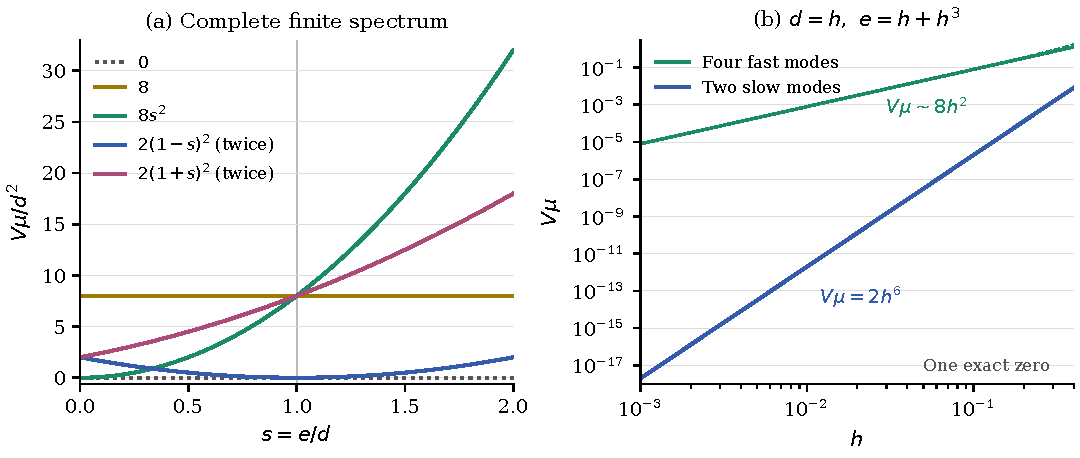
\includegraphics[width=\textwidth]{output/figures/two_cycle_spectrum.pdf}
 \caption{The exact finite spectrum in \eqref{eq:two-cycle-spectrum}.
 Panel (a) shows all seven eigenvalues, with the two double
 branches labelled. At $e=d>0$ the kernel has dimension three.
 Panel (b) takes $d=h$, $e=h+h^3$: two modes have scale
 $h^6$, four have scale $h^2$, and one is exactly zero.
 These are finite matrix calculations. The relative theorem
 transfers their asymptotics to the actual HYM linearization.}
 \label{fig:two-cycle}
\end{figure}

Figure~\ref{fig:two-cycle} also illustrates why the size
of the arrows alone does not determine the weakest rates.
The linear relaxation time of the two difference modes is
of order $h^{-2b}$. An approximation of nonlinear
trajectories on such intervals requires more than the
spectral comparison. The next three sections construct
the exact finite evolution and the phase selected by a
spatially varying initial metric.
